% Substituição da Nota Editorial 1 — Seção 5.1 (Painéis Metodológicos Controlados)
\begin{figure}[htbp]
  \centering
  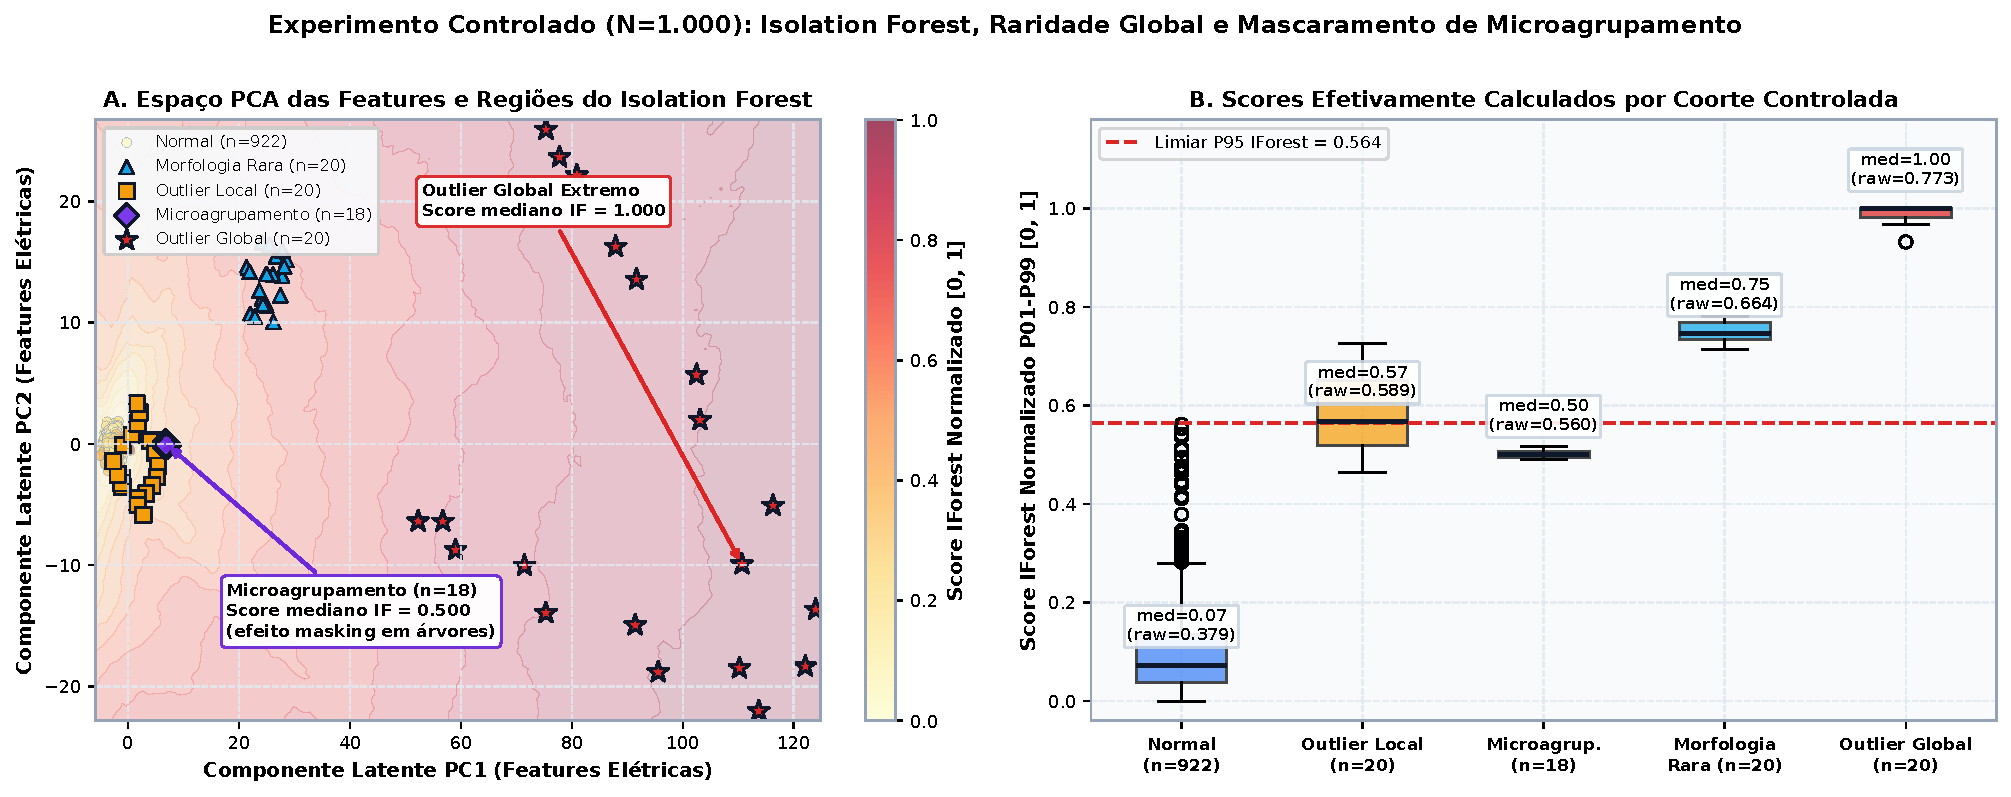
\includegraphics[width=0.98\textwidth]{manuscript_figures/ml_controlled_panels/fig_5_1a_isolation_forest_microcluster.pdf}
  \caption{Experimento controlado ($N=1.000$, \texttt{seed=42}): projeção PCA dos escores efetivamente calculados pelo \emph{Isolation Forest} e distribuição por coorte geradora, ilustrando a atenuação do escore no microagrupamento compacto ($n=18$) por compartilhamento de partições (\emph{masking}).}
  \label{fig:ml-iforest-microcluster}
\end{figure}

\begin{figure}[htbp]
  \centering
  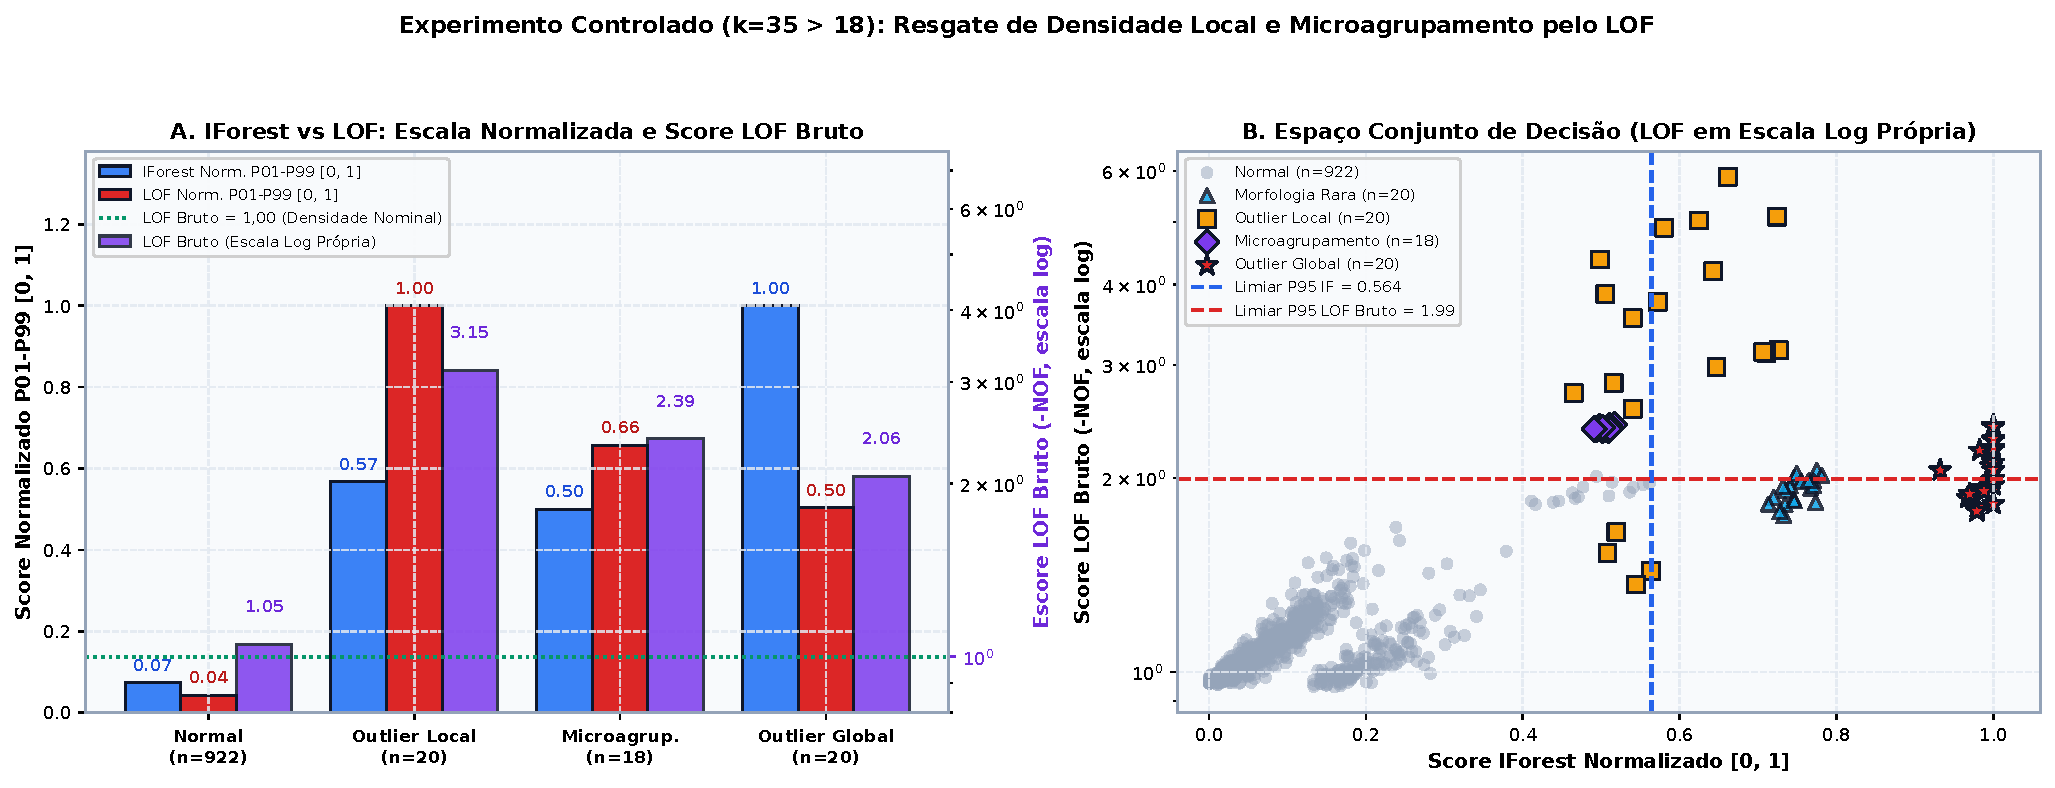
\includegraphics[width=0.98\textwidth]{manuscript_figures/ml_controlled_panels/fig_5_1b_lof_escala_propria.pdf}
  \caption{Respostas do \emph{Local Outlier Factor} ($k=35 > 18$) no experimento controlado ($N=1.000$): (A) contraste em escala bruta logarítmica própria ($-\text{NOF}$) e normalizada por quantis P01--P99 $[0,1]$; (B) espaço de decisão conjunto com \emph{Isolation Forest} destacando os quadrantes de recuperação do outlier local e do microagrupamento.}
  \label{fig:ml-lof-escala-propria}
\end{figure}

\begin{figure}[htbp]
  \centering
  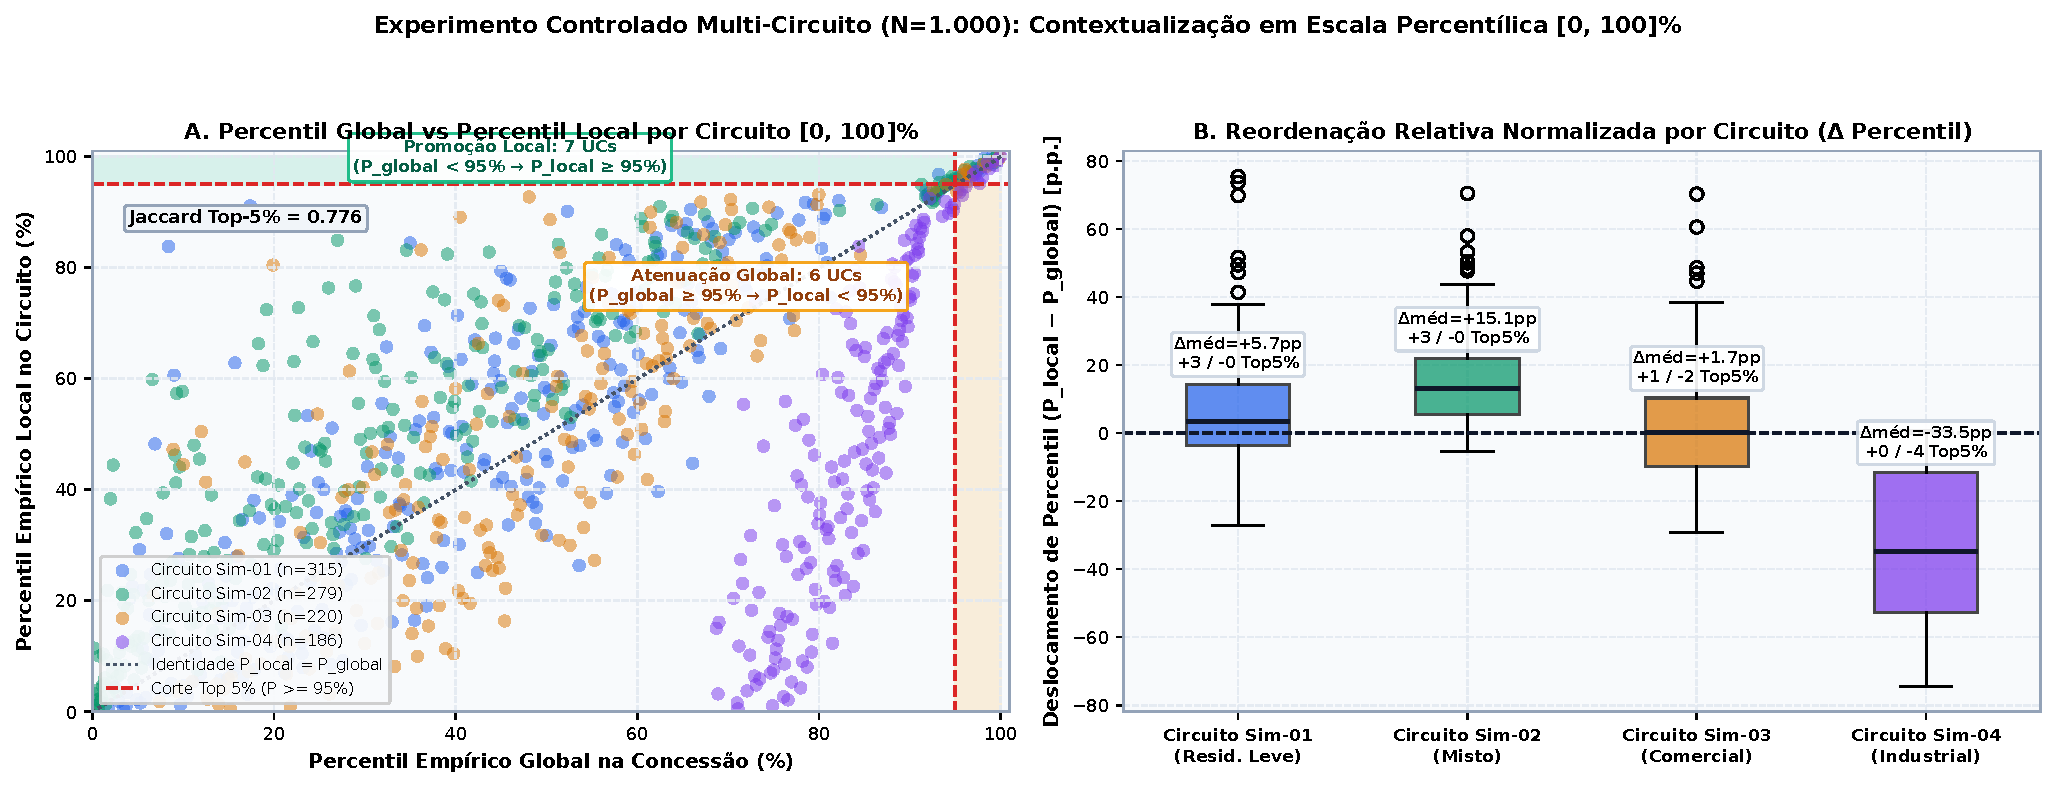
\includegraphics[width=0.98\textwidth]{manuscript_figures/ml_controlled_panels/fig_5_1c_contextualizacao_percentis.pdf}
  \caption{Contextualização por circuito elétrico no experimento controlado ($N=1.000$) em escala normalizada de percentis $[0,100]\%$: (A) percentil empírico global versus percentil empírico local intra-circuito com limiar $P_{95}$; (B) deslocamento líquido de percentil ($\Delta P = P_{\text{local}} - P_{\text{global}}$) por perfil de circuito.}
  \label{fig:ml-contextualizacao-percentis}
\end{figure}

Nos três painéis controlados (\texttt{seed=42}, $N=1.000$), os parâmetros geradores são conhecidos apenas para verificação mecanística dos algoritmos, não devendo ser confundidos com estatísticas da rede real. A Figura~\ref{fig:ml-iforest-microcluster} mostra que o microagrupamento compacto ($n=18$) reduz a facilidade de isolamento recursivo em árvores aleatórias, mantendo sua mediana abaixo do corte $P_{95}$ e de outliers globais isolados. Na Figura~\ref{fig:ml-lof-escala-propria}, o uso de escala bruta própria ($-\text{NOF}$ em escala logarítmica) combinada à padronização quantílica P01--P99 evita achatamento visual e demonstra que, quando $k=35$ excede o tamanho do microagrupamento, tanto desvios locais quanto o grupo compacto recebem pontuação LOF bruta acima de $P_{95}$. Por fim, a Figura~\ref{fig:ml-contextualizacao-percentis} substitui posições ordinais dependentes de tamanho amostral por comparação direta entre percentis empíricos global e local $[0,100]\%$, explicitando promoções em circuitos residenciais leves e atenuações de cargas nominais elevadas em circuitos industriais.
